\subsection*{Problema 07}

\textbf{Enunciado:} Evaluar la integral definida 
mediante sumas de Riemann:
\begin{align*}
\int_{-1}^{1} x \, dx
\end{align*}

\textbf{Solución:} 
Para evaluar la integral usando la definición 
de la suma de Riemann, consideramos el intervalo 
$[a, b] = [-1, 1]$ con una partición regular 
de $n$ subintervalos de igual ancho $\Delta x$.

El ancho de cada subintervalo es:
\begin{align*}
\Delta x &= \dfrac{b - a}{n} \\
&= \dfrac{1 - (-1)}{n} = \dfrac{2}{n}
\end{align*}

Tomamos el extremo derecho de cada subintervalo 
como punto muestra $x_i$:
\begin{align*}
x_i &= a + i \Delta x \\
&= -1 + i \left(\dfrac{2}{n}\right)
\end{align*}

Evaluamos la función $f(x) = x$ en cada $x_i$:
\begin{align*}
f(x_i) &= -1 + \dfrac{2i}{n}
\end{align*}

Planteamos la suma de Riemann usando el 
límite cuando $n \to \infty$:
\begin{align*}
\int_{-1}^{1} x \, dx &= \lim_{n \to \infty} 
\sum_{i=1}^{n} f(x_i) \Delta x
\end{align*}

Sustituimos $f(x_i)$ y $\Delta x$:
\begin{align*}
\int_{-1}^{1} x \, dx &= \lim_{n \to \infty} 
\sum_{i=1}^{n} \left( -1 + \dfrac{2i}{n} \right) 
\left( \dfrac{2}{n} \right)
\end{align*}

Expandimos la expresión algebraica dentro 
de la sumatoria:
\begin{align*}
&= \lim_{n \to \infty} \dfrac{2}{n} \sum_{i=1}^{n} 
\left( -1 + \dfrac{2i}{n} \right) \\
&= \lim_{n \to \infty} \dfrac{2}{n} \left[ 
\sum_{i=1}^{n} (-1) + \dfrac{2}{n} \sum_{i=1}^{n} i 
\right]
\end{align*}

Aplicamos las fórmulas de sumas notables 
$\sum_{i=1}^{n} 1 = n$ y $\sum_{i=1}^{n} i = \dfrac{n(n+1)}{2}$:
\begin{align*}
&= \lim_{n \to \infty} \dfrac{2}{n} \left[ 
-n + \dfrac{2}{n} \left( \dfrac{n(n+1)}{2} \right) 
\right]
\end{align*}

Simplificamos algebraicamente:
\begin{align*}
&= \lim_{n \to \infty} \dfrac{2}{n} \left[ 
-n + (n + 1) \right] \\
&= \lim_{n \to \infty} \dfrac{2}{n} (1) \\
&= \lim_{n \to \infty} \dfrac{2}{n} = 0
\end{align*}

Por lo tanto, el valor de la integral definida es:
\begin{align*}
\int_{-1}^{1} x \, dx = 0
\end{align*}

\begin{figure}[H]
	\centering
	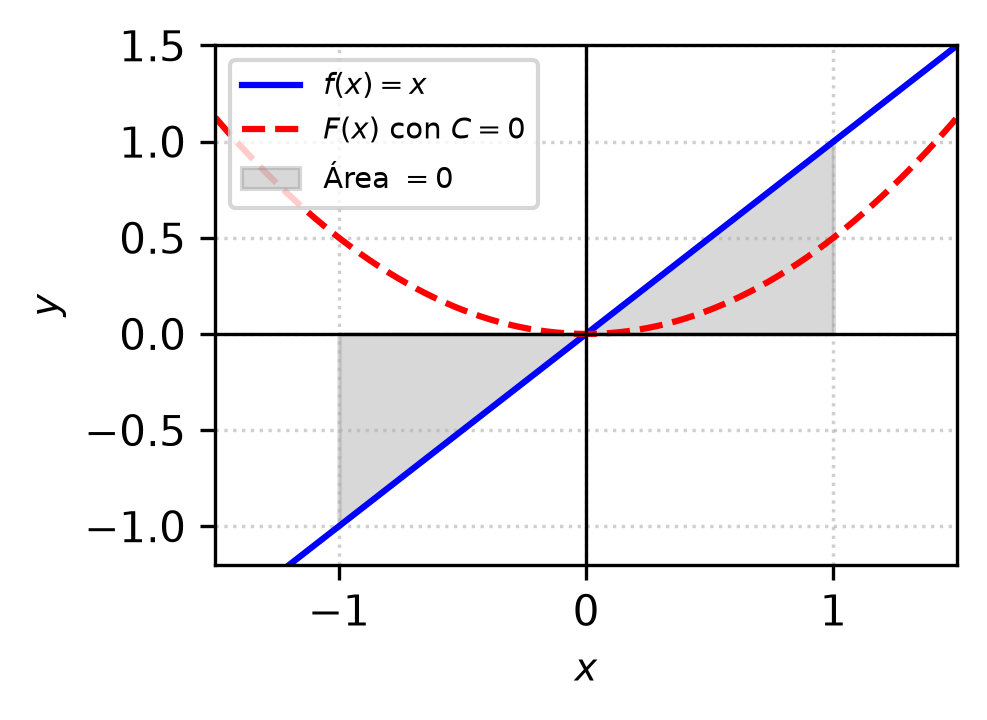
\includegraphics[width=\columnwidth]{semana_06/graficas/SEM06_P07_grafica.png}
	\caption{Representación gráfica de $f(x)$ y su antiderivada $F(x)$ evaluada para la constante de integración $C = 0$ (Problema 07).}
	\label{fig:problema07}
\end{figure}
